\documentclass[conference]{IEEEtran}

\usepackage[T1]{fontenc}
\usepackage{graphicx}
\usepackage{booktabs}
\usepackage{cite}
\usepackage{url}
\usepackage{balance}
\usepackage[hidelinks]{hyperref}

\title{CropVision: Comparing Traditional Machine Learning and a Convolutional Neural Network for Satellite Image Classification}

\author{
\IEEEauthorblockN{Malik SAADI, Edgar PRADET, Etienne SIOEN}
\IEEEauthorblockA{
\textit{School of Computer Science, Hanyang University (exchange)}\\
Seoul, Republic of Korea\\
\{malik.saadi, edgar.pradet\}@edu.ece.fr, etienne.sioen@edu.devinci.fr}
}

\begin{document}

\maketitle

\begin{abstract}
This paper compares traditional machine-learning pipelines with a compact
convolutional neural network (CNN) for classifying EuroSAT RGB satellite
images. We use a deterministic, stratified 70/15/15 split of 27,000 images and
evaluate Random Forest, Random Forest with principal component analysis (PCA),
an RBF support vector machine (SVM) with PCA, and a custom CNN. Model and
checkpoint selection use only the training and validation partitions. The four
frozen models are then evaluated once on the same 4,050-image test set. The CNN
achieves 93.88\% test accuracy and 0.9369 macro-F1, substantially outperforming
the traditional models, which obtain 67.23--68.47\% accuracy and
0.6599--0.6695 macro-F1. PCA reduces computation but does not improve final
Random Forest accuracy. The results show the advantage of learned spatial
features for this RGB patch-classification task, while also illustrating the
importance of leakage prevention, resource-aware experiment design, and
class-level error analysis.
\end{abstract}

\begin{IEEEkeywords}
satellite imagery, EuroSAT, land-use classification, random forest, support
vector machine, principal component analysis, convolutional neural network
\end{IEEEkeywords}

\section{Introduction}

Earth-observation imagery supports applications in agriculture,
environmental monitoring, and urban planning. Its growing volume makes manual
land-use interpretation difficult to scale. Machine learning can automate this
task, but model families use image information differently. Traditional
classifiers generally require an explicit feature vector, whereas deep neural
networks can learn spatial representations directly from pixels.

CropVision addresses the question: \emph{How do traditional machine-learning
methods and a deep-learning approach compare in satellite image
classification?} We compare three traditional pipelines against a compact CNN
under a common data split and evaluation protocol. The objective is not to
claim a new state of the art, but to study predictive performance,
class-specific behavior, runtime, and practical constraints in a reproducible
undergraduate engineering project. Our contributions are: (1) a validated,
leakage-safe EuroSAT RGB workflow; (2) comparable Random Forest, PCA, SVM, and
CNN experiments; and (3) a one-shot held-out test evaluation with saved
provenance and figures.

\section{Datasets}

We use the RGB release of EuroSAT, a benchmark derived from Sentinel-2 images
over European locations \cite{helber2019}. It contains 27,000 JPEG patches of
size $64\times64$ pixels in ten land-use and land-cover classes: AnnualCrop,
Forest, HerbaceousVegetation, Highway, Industrial, Pasture, PermanentCrop,
Residential, River, and SeaLake. Class sizes range from 2,000 Pasture images to
3,000 images in five classes. Only visible RGB channels are used; the 13-band
multispectral dataset is outside this study.

The documented archive was checksum-verified, and all images were decoded to
confirm RGB mode, shape, and class counts. Using seed 42, we created a
stratified 70/15/15 partition: 18,900 training, 4,050 validation, and 4,050
test images. An identity audit found no overlap between any pair of partitions,
no missing files, and no unknown manifest paths. The validation set was used
for candidate and checkpoint selection. Training programs did not decode test
images; the test partition was used only after all configurations were frozen.

\begin{table}[t]
\centering
\caption{Deterministic EuroSAT RGB partition (seed 42).}
\label{tab:split}
\footnotesize
\begin{tabular}{lrr}
\toprule
Partition & Fraction & Images \\
\midrule
Training   & 70\% & 18,900 \\
Validation & 15\% & 4,050 \\
Test       & 15\% & 4,050 \\
\midrule
Total      & 100\% & 27,000 \\
\bottomrule
\end{tabular}
\end{table}

\section{Methodology}

\subsection{Shared Protocol}

All models use the same image identities, class order, and seed. Selection is
based on validation macro-F1 so that each class contributes equally despite
the moderate imbalance. Learned scalers, PCA projections, and normalization
statistics are fitted or calculated exclusively from training images.

For classical models, RGB values are scaled to $[0,1]$ and flattened into
12,288-dimensional float vectors. This is a simple reproducible baseline, but
it discards explicit two-dimensional neighborhood information. Each selected
scikit-learn pipeline remains fitted only on the training partition.

\subsection{Traditional Models}

The Random Forest baseline follows Breiman's ensemble principle
\cite{breiman2001}. Two bounded candidates were compared. The selected model
uses 300 trees, unlimited depth, one minimum sample per leaf,
\texttt{max\_features=sqrt}, and seed 42. No scaling is required because tree
split decisions are invariant to feature scale.

PCA projects correlated features onto orthogonal directions of decreasing
variance \cite{pearson1901}. The Random Forest + PCA pipeline first applies a
training-fitted standard scaler, then randomized PCA with 128 components, and
finally the same forest candidate search. This reduces 12,288 inputs to 128
components while keeping preprocessing inside the fitted pipeline.

SVMs construct maximum-margin boundaries and can model nonlinear separation
through kernels \cite{cortes1995}. Our feasible full-data pipeline applies the
same scaling and 128-component PCA before an RBF SVM. We evaluated
$C\in\{1,10\}$ with \texttt{gamma=scale}; validation macro-F1 selected
$C=10$. A full raw-pixel RBF SVM was \emph{not} trained because its kernel
calculation and support-vector footprint were not suitable for the available
8~GB Apple Silicon Mac. A reduced subset was not presented as a full-data
result.

Table~\ref{tab:configurations} summarizes the frozen representations and
selected settings. The deliberately small candidate grids kept selection runs
feasible on the target computer. PCA and scaling remained pipeline steps and
were never calculated before the data split.

\begin{table}[t]
\centering
\caption{Model configurations selected on validation macro-F1.}
\label{tab:configurations}
\footnotesize
\setlength{\tabcolsep}{3.5pt}
\begin{tabular}{lp{1.05cm}p{3.55cm}}
\toprule
Model & Input & Selected setting \\
\midrule
RF & 12,288 px & 300 trees, unlimited depth, \texttt{sqrt} features \\
RF + PCA & 128 PCs & StandardScaler, randomized PCA, same RF \\
SVM + PCA & 128 PCs & StandardScaler, randomized PCA, RBF, $C=10$ \\
CNN & RGB tensor & 32/64/128 channels, 256-unit head, 30\% dropout \\
\bottomrule
\end{tabular}
\end{table}

\subsection{Convolutional Neural Network}

Convolutional networks learn local spatial patterns using shared filters
\cite{lecun1998}. Our 620,362-parameter CNN contains three
convolution--ReLU--max-pooling blocks with 32, 64, and 128 output channels.
Adaptive average pooling produces a $128\times4\times4$ representation. The
classification head contains a 256-unit linear layer, ReLU, 30\% dropout, and
ten output logits.

Channel means $(0.3439,0.3801,0.4078)$ and standard deviations
$(0.2024,0.1369,0.1158)$ were computed from training identities only. Training
used cross-entropy loss and Adam \cite{kingma2015} with learning rate 0.001,
weight decay $10^{-4}$, batch size 64, and at most 30 epochs. Seeds were fixed
for Python, NumPy, and PyTorch. The code supports Apple MPS with CPU fallback;
the recorded full run used CPU. Checkpoints were selected by validation
macro-F1, with early-stopping patience five. Training stopped after 26 epochs,
and epoch 21 was retained.

\section{Evaluation \& Analysis}

Before test evaluation, model steps, hyperparameters, selected candidate or
epoch, validation scores, artifact paths, and SHA-256 hashes were frozen. A
separate evaluator verified these records and scored the same test manifest
without retraining. Table~\ref{tab:results} distinguishes validation selection
scores from the final held-out results.

Accuracy measures the overall proportion of correct predictions. Macro-F1 is
the unweighted mean of the ten class F1-scores and is less dominated by larger
classes. We also calculated macro precision, macro recall, per-class metrics,
confusion matrices, and inference time. The evaluator wrote a persistent state
after the approved run, preventing a silent second test evaluation. This
separation reduces the risk of adapting decisions to test feedback.

\begin{figure*}[t]
\centering
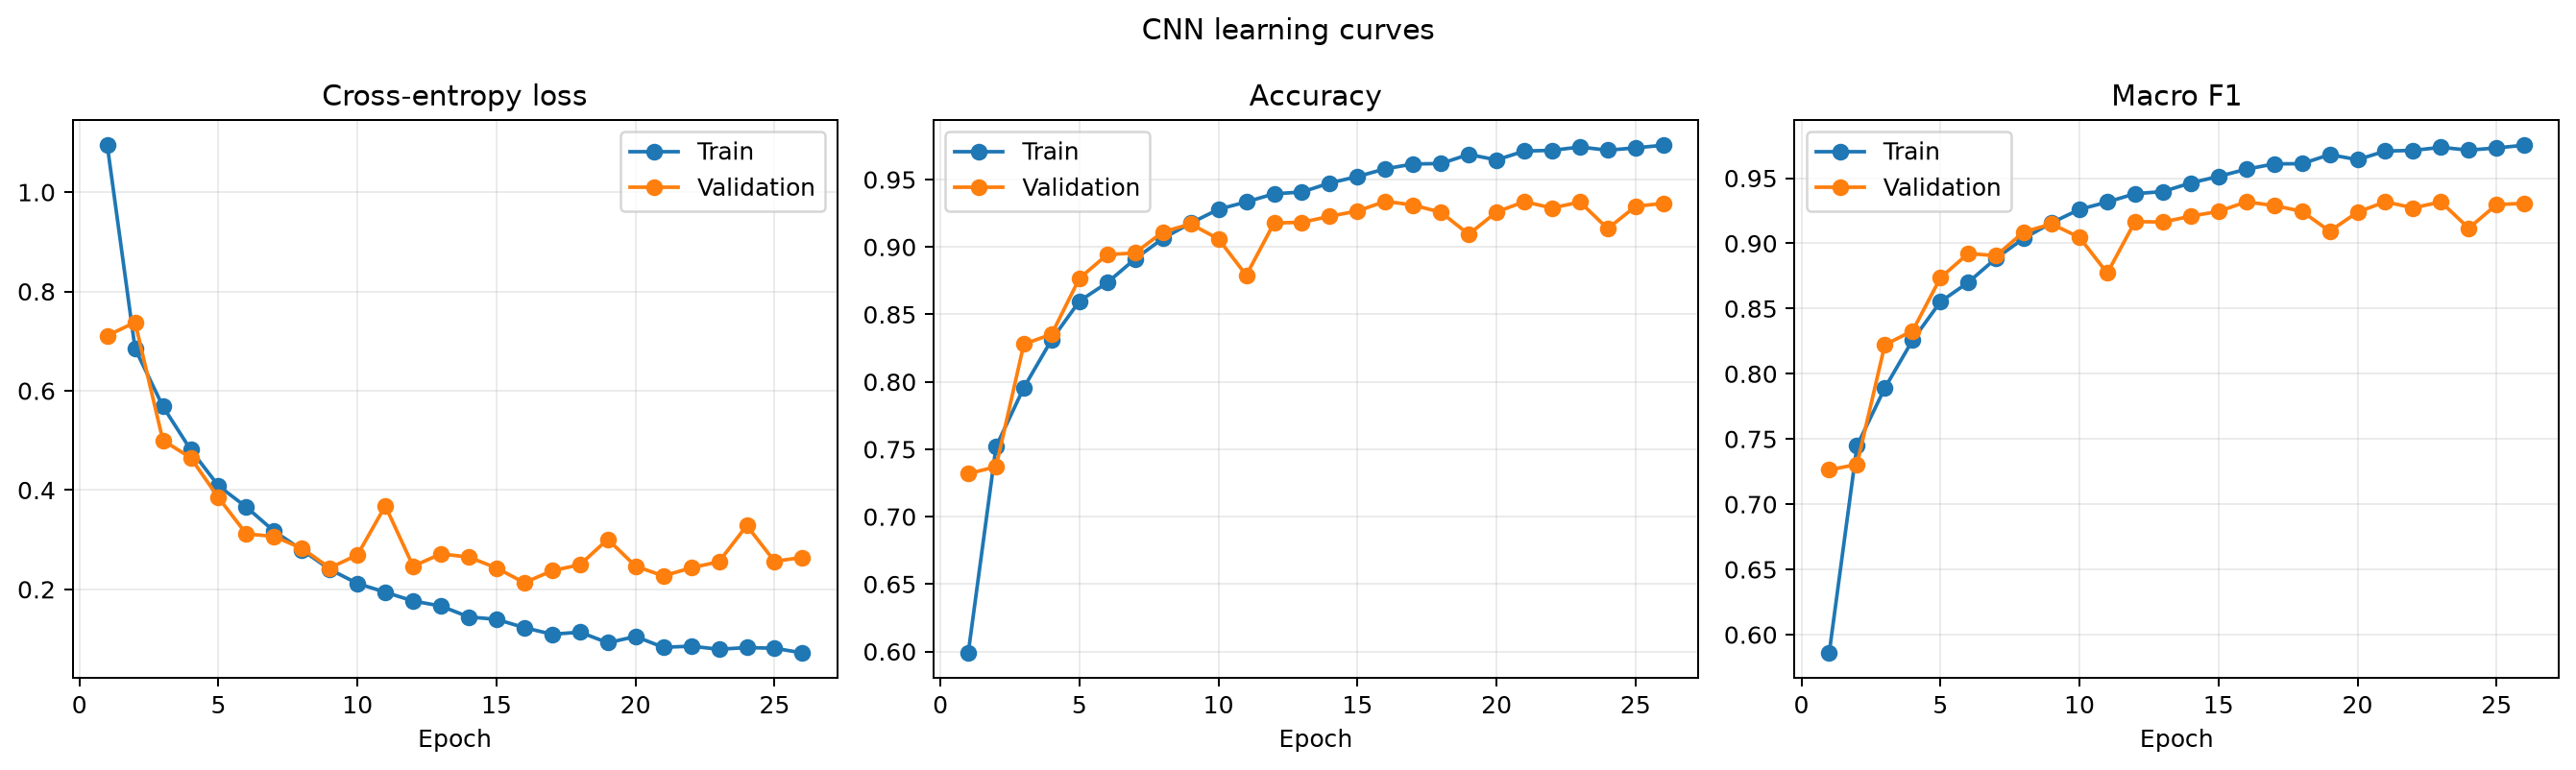
\includegraphics[width=0.96\textwidth]{../../results/figures/cnn/full_cnn_phase4_20261115_v2/learning_curves.png}
\caption{CNN training and validation curves. The epoch-21 checkpoint maximizes validation macro-F1; later loss divergence indicates moderate overfitting.}
\label{fig:learning-curves}
\end{figure*}

\begin{table*}[t]
\centering
\caption{Validation and final held-out test results. Inference excludes JPEG decoding.}
\label{tab:results}
\small
\setlength{\tabcolsep}{7pt}
\begin{tabular}{lccccc}
\toprule
Model & Val. Accuracy & Val. Macro-F1 & Test Accuracy & Test Macro-F1 & Inference (s) \\
\midrule
Random Forest       & 68.00\% & 0.6627 & 68.47\% & 0.6695 & 0.247 \\
Random Forest + PCA & 68.30\% & 0.6621 & 67.90\% & 0.6599 & \textbf{0.202} \\
SVM + PCA           & 67.09\% & 0.6619 & 67.23\% & 0.6632 & 3.449 \\
\textbf{CNN}        & \textbf{93.36\%} & \textbf{0.9318} & \textbf{93.88\%} & \textbf{0.9369} & 3.519 \\
\bottomrule
\end{tabular}
\end{table*}

\begin{figure}[t]
\centering
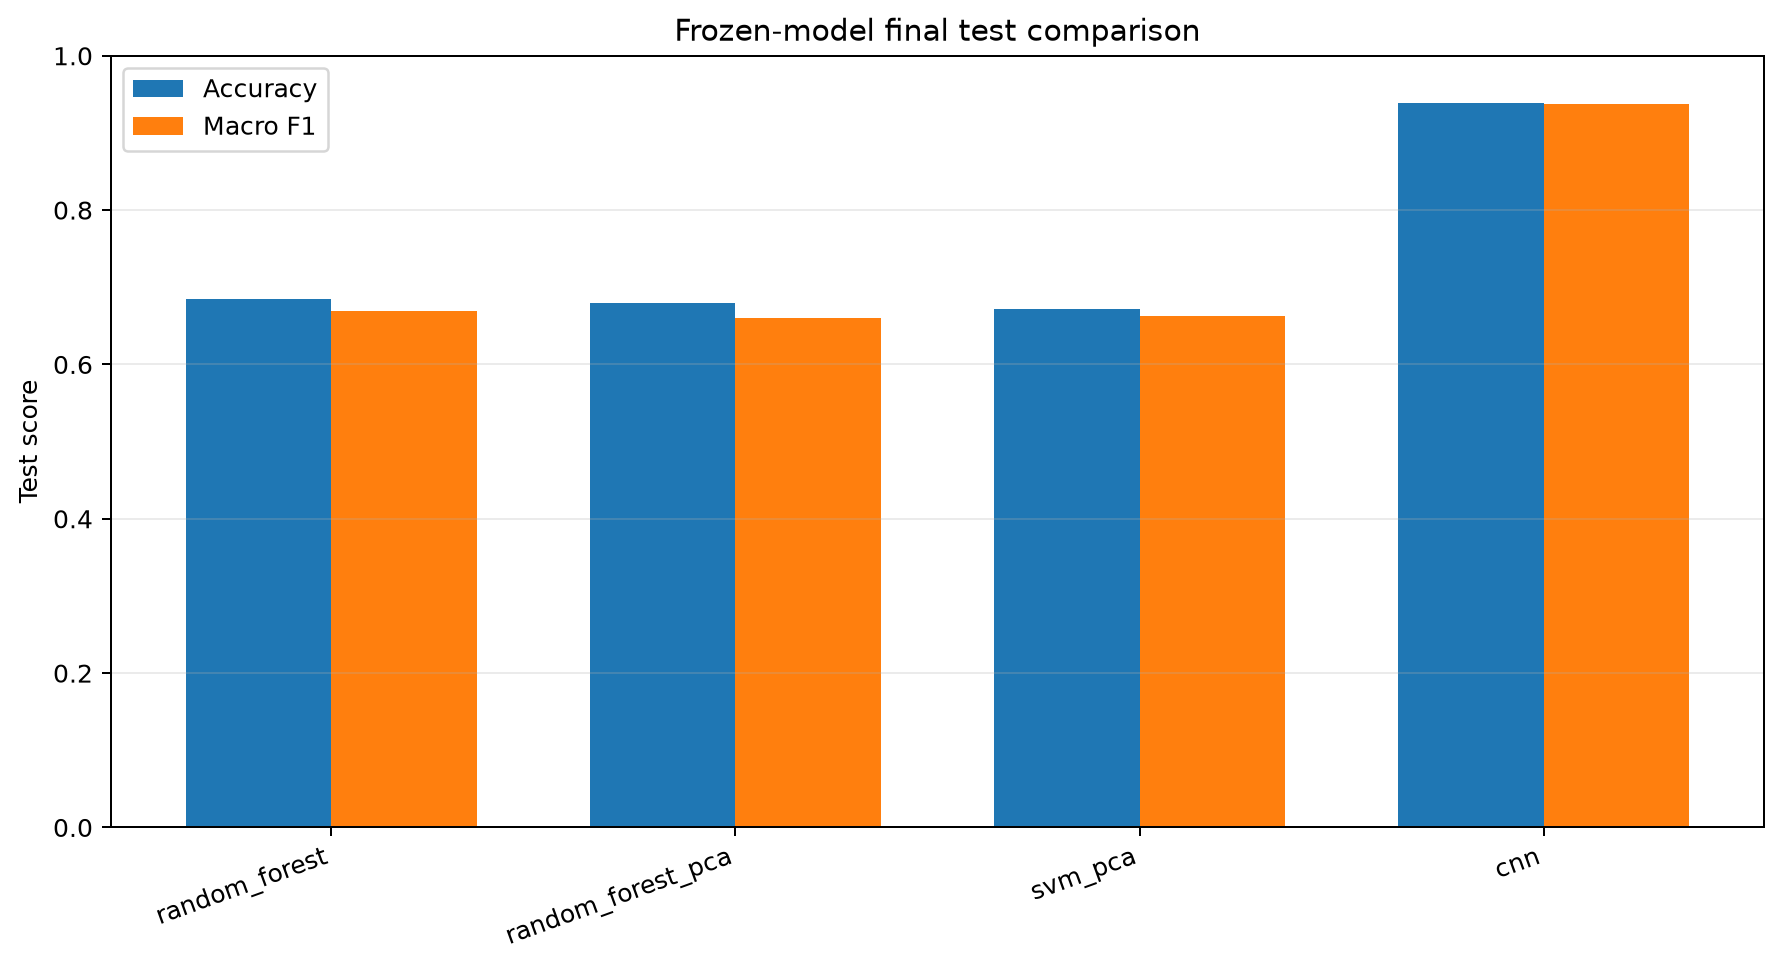
\includegraphics[width=\columnwidth]{../../results/figures/final/final_test_phase5/test_comparison.png}
\caption{Accuracy and macro-F1 on the 4,050-image held-out test set.}
\label{fig:test-comparison}
\end{figure}

The CNN improves test accuracy by 25.41 percentage points and macro-F1 by
26.74 points over the strongest traditional result, Random Forest. The
validation-to-test differences for all models remain below one percentage
point, which is consistent with the fixed split and validation-only selection
procedure. Figure~\ref{fig:test-comparison} summarizes the performance gap.

The traditional models perform best on visually distinctive categories.
Random Forest test F1 reaches 0.9293 for SeaLake and 0.8814 for Forest, but only
0.3882 for Highway and 0.4690 for PermanentCrop. Highway recall is 29.87\%; its
images are often predicted as Residential, AnnualCrop, or River. Flattened
color values do not explicitly describe road continuity, field boundaries, or
repeating crop structure. PCA does not improve the forest's final result:
accuracy decreases from 68.47\% to 67.90\%, and macro-F1 from 0.6695 to 0.6599.

The CNN exceeds 0.90 F1 for every class. SeaLake is highest at 0.9716, followed
by Residential at 0.9682. Pasture is lowest at 0.9005: recall is 95.00\%, but
precision is 85.59\%. Remaining confusions are plausible for small RGB patches:
19 Forest images are predicted as Pasture, 19 PermanentCrop images as
HerbaceousVegetation, and 14 Highway images as River.

\begin{table}[t]
\centering
\caption{Per-class F1 on the held-out test set.}
\label{tab:per-class}
\footnotesize
\setlength{\tabcolsep}{3.6pt}
\begin{tabular}{lrrrr}
\toprule
Class & RF & RF+PCA & SVM+PCA & CNN \\
\midrule
AnnualCrop    & .6771 & .6336 & .6085 & \textbf{.9369} \\
Forest        & .8814 & .9258 & .8703 & \textbf{.9607} \\
Herbaceous    & .5847 & .5910 & .6002 & \textbf{.9163} \\
Highway       & .3882 & .3452 & .3988 & \textbf{.9199} \\
Industrial    & .8068 & .8171 & .8432 & \textbf{.9626} \\
Pasture       & .7234 & .7452 & .7011 & \textbf{.9005} \\
PermanentCrop & .4690 & .4349 & .5125 & \textbf{.9144} \\
Residential   & .6131 & .6565 & .6728 & \textbf{.9682} \\
River         & .6220 & .5442 & .6008 & \textbf{.9180} \\
SeaLake       & .9293 & .9059 & .8235 & \textbf{.9716} \\
\bottomrule
\end{tabular}
\end{table}

Figure~\ref{fig:learning-curves} shows moderate overfitting. At the selected
epoch, training accuracy is 97.11\% and validation accuracy is 93.36\%, with
validation loss 0.2269. By epoch 26, training accuracy increases to 97.54\%,
while validation accuracy remains 93.23\% and validation loss rises to 0.2643.
Checkpointing therefore prevents later epochs from replacing the better
validation model.

Runtime measurements provide context rather than a strict cross-framework
benchmark. The selected Random Forest, Random Forest + PCA, and SVM + PCA fits
took 76.64, 25.05, and 9.72~s, respectively, excluding classical feature-cache
creation. CNN training took 1,213.53~s (20~min 14~s) for 26 CPU epochs. PCA
substantially reduces forest fitting time, but does not increase test accuracy.
Final classical inference includes pipeline transformation and prediction,
whereas CNN timing measures forward passes over preloaded normalized tensors;
JPEG decoding is excluded from both.

\section{Related Work}

EuroSAT was introduced as a Sentinel-2 benchmark for land-use and land-cover
classification \cite{helber2019}. Sentinel-2 itself is a high-resolution
optical Earth-observation mission designed for operational land services
\cite{drusch2012}. The original EuroSAT study includes multispectral data and
deep networks, so its reported values are not directly comparable to our
RGB-only split and compact architecture.

CropVision combines established statistical learning methods
\cite{breiman2001,cortes1995,pearson1901} with a CNN that learns spatial
features directly from pixels \cite{lecun1998}. This follows the broader move
toward representation learning in remote sensing described by Zhu et al.
\cite{zhu2017}. Our experiment is deliberately smaller than modern
state-of-the-art studies: it emphasizes a controlled, resource-aware comparison
rather than transfer learning or large-scale architecture search.

\section{Conclusion \& Discussion}

For the selected EuroSAT RGB split, the compact CNN clearly outperforms the
traditional raw-pixel pipelines, reaching 93.88\% test accuracy and 0.9369
macro-F1. Random Forest is the strongest traditional test model at 68.47\%
accuracy and 0.6695 macro-F1. PCA makes full-data nonlinear SVM training
manageable and reduces forest fitting time, but does not improve the forest's
held-out score. The results support the value of preserving spatial structure
for satellite image classification.

Several limitations prevent broad generalization. Only RGB channels are used;
the split is stratified rather than geographically separated; and results come
from one seed and one dataset without confidence intervals. Hyperparameter
search is intentionally limited for an 8~GB Mac. The CNN uses no augmentation,
transfer learning, or learning-rate schedule. A full raw-pixel RBF SVM is
absent, and recorded timing scopes differ between frameworks. Finally,
classifying isolated $64\times64$ patches is not equivalent to semantic
segmentation or deployment on new regions.

Future work should evaluate geographic group splits, repeated seeds,
multispectral bands, calibrated uncertainty, engineered texture features, and
resource-aware linear SVMs. The complete source, frozen configurations,
metrics, figures, and reproduction instructions are available at
\url{https://github.com/Malik010605/CropVision}. Large datasets and model
checkpoints are intentionally excluded but can be regenerated from the
documented workflow.

\balance
\begin{thebibliography}{00}

\bibitem{helber2019}
P. Helber, B. Bischke, A. Dengel, and D. Borth, ``EuroSAT: A novel dataset and
deep learning benchmark for land use and land cover classification,''
\emph{IEEE J. Sel. Topics Appl. Earth Observ. Remote Sens.}, vol. 12, no. 7,
pp. 2217--2226, 2019, doi: 10.1109/JSTARS.2019.2918242.

\bibitem{drusch2012}
M. Drusch \emph{et al.}, ``Sentinel-2: ESA's optical high-resolution mission
for GMES operational services,'' \emph{Remote Sens. Environ.}, vol. 120,
pp. 25--36, 2012, doi: 10.1016/j.rse.2011.11.026.

\bibitem{breiman2001}
L. Breiman, ``Random forests,'' \emph{Mach. Learn.}, vol. 45, pp. 5--32, 2001,
doi: 10.1023/A:1010933404324.

\bibitem{cortes1995}
C. Cortes and V. Vapnik, ``Support-vector networks,'' \emph{Mach. Learn.},
vol. 20, pp. 273--297, 1995, doi: 10.1007/BF00994018.

\bibitem{pearson1901}
K. Pearson, ``On lines and planes of closest fit to systems of points in
space,'' \emph{Philos. Mag.}, vol. 2, no. 11, pp. 559--572, 1901,
doi: 10.1080/14786440109462720.

\bibitem{lecun1998}
Y. LeCun, L. Bottou, Y. Bengio, and P. Haffner, ``Gradient-based learning
applied to document recognition,'' \emph{Proc. IEEE}, vol. 86, no. 11,
pp. 2278--2324, 1998, doi: 10.1109/5.726791.

\bibitem{kingma2015}
D. P. Kingma and J. Ba, ``Adam: A method for stochastic optimization,'' in
\emph{Proc. 3rd Int. Conf. Learn. Representations (ICLR)}, 2015.

\bibitem{zhu2017}
X. X. Zhu \emph{et al.}, ``Deep learning in remote sensing: A comprehensive
review and list of resources,'' \emph{IEEE Geosci. Remote Sens. Mag.}, vol. 5,
no. 4, pp. 8--36, 2017, doi: 10.1109/MGRS.2017.2762307.

\end{thebibliography}

\end{document}
